\FloatBarrier

\section{Synthetic data: trainable MLP}
\label{sec:mlp}

The RFNN microscope predicts that widening the latent space separates the slowest population mode from the fastest sample-specific mode by a factor that grows with $\dlat$ (Sec.~\ref{sec:theory-buffer}). We next test the same mechanism in a trainable score network. The synthetic MLP uses the same Gaussian-mixture data as the RFNN experiment, but the first layer is learned and the score is trained over diffusion times. Additional controls for width, learning rate, optimizer choice, and robustness settings are reported in the appendix.

The main-text synthetic MLP sweep uses $\dint=5$, $n=500$ training samples, null-noise scale $\sigma_\perp=0.5$, $\dlat\in \{5,8,10,12,15,20,25,30,35,40\}$, and seeds 42--46. Each model is trained for 5M steps with hidden width fixed at 256. We count a generated sample as memorized when its nearest-neighbor ratio is below $1/3$, following the ratio test of \citet{somepalli2023diffusion} and the threshold used by \citet{bonnaire2025}. For the synthetic quality analogue of FID, we report analytic score error normalized per latent dimension, recomputed with the corrected metric (the released curves used $Q^\top D^{-1}Q$ in place of $QD^{-1}Q^\top$ and are not reported); Sec.~\ref{sec:theory-linear} gives a parameter-free prediction of the initial value $[J_S+(\dlat-\dint)/\beta_t^2]/\dlat$ and of the late-time shape., since the target GMM score is known exactly and output-size scaling should not masquerade as a quality trend. The full memorization trajectories and raw score-error curves are in Appendix~\ref{app:synthetic-mlp-clean}, Figures~\ref{fig:app-synthetic-mlp-mem} and \ref{fig:app-synthetic-mlp-score}; there we extend the same fixed-width sweep through $\dlat=240$ and report peak memorization across the run.

\begin{figure*}[!t]
  \centering
  \begin{subfigure}{0.44\textwidth}
    \centering
    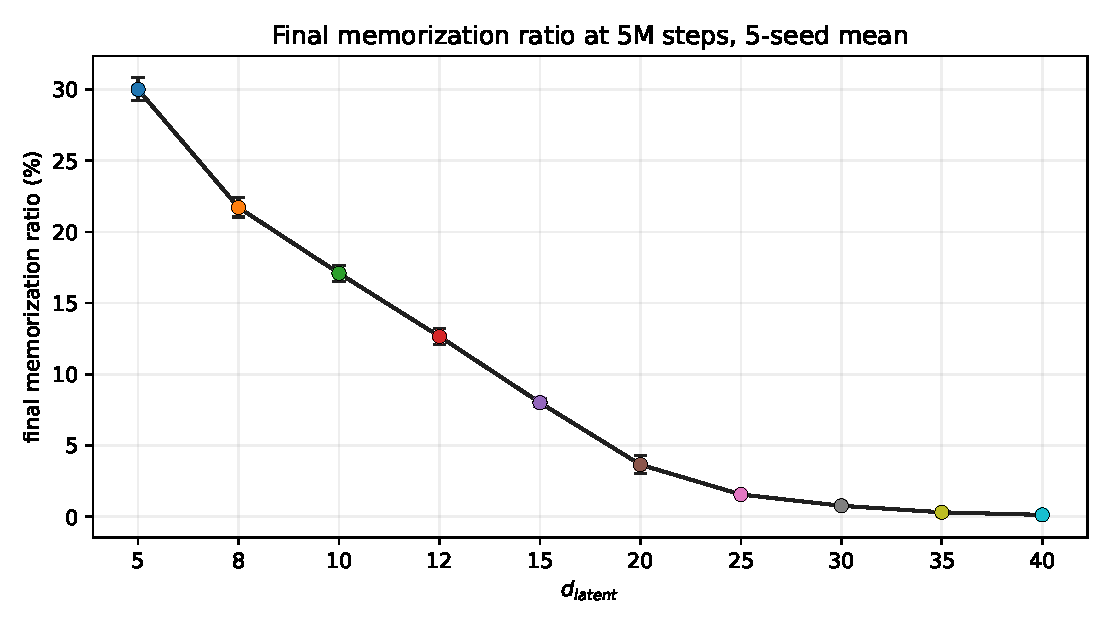
\includegraphics[width=\linewidth]{figures/synthetic_mlp_final_mem_ratio.pdf}
    \caption{Final memorization.}
    \label{fig:synthetic-mlp-final-mem}
  \end{subfigure}\hfill
  \begin{subfigure}{0.52\textwidth}
    \centering
    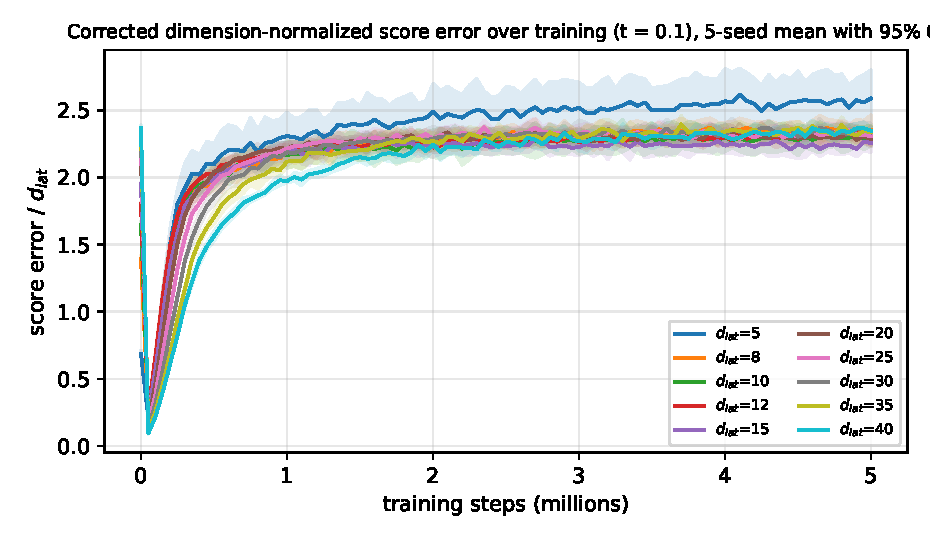
\includegraphics[width=\linewidth]{figures/synthetic_mlp_score_error_per_dim.pdf}
    \caption{Dimension-normalized score error.}
    \label{fig:synthetic-mlp-score-error}
  \end{subfigure}
  \caption{\textbf{Synthetic MLP memorization and quality.}
    Five-seed fixed-width MLP results after or during 5M steps, sweeping
    $\dlat$ at exact $\dint=5$. Once $\dlat$ exceeds the intrinsic dimension, final memorization falls monotonically from $30\%$ at $\dlat=5$ to $0.1\%$ at $\dlat=40$, with hidden width $256$ at every $\dlat$ (\cref{fig:app-synthetic-mlp-scaled} shows the same sweep with width scaled as $8\dlat$). The score-error panel is the population score error at $t=0.1$ per coordinate, against the exact GMM score on held-out data. Every width reaches its minimum by the first evaluation at 50k steps and then diverges from the population score as the network fits its training set. The divergence starts later at larger $\dlat$: the error crosses $2.0$ per coordinate at $0.35$M steps for $\dlat=5$ and at $1.05$M for $\dlat=40$, the same ordering as the memorization onset. By 5M steps all widths have diverged to a similar level, so the panel shows the delay, not a preserved score at the horizon.}
  \label{fig:synthetic-mlp-main}
\end{figure*}

On synthetic data the population score error is available exactly, so it replaces FID as the quality readout. It does not show quality preserved at the 5M-step horizon; every width has left the population score by then. What it shows is timing: the divergence from the population score, which is the score-space signature of fitting the training set, begins about $3\times$ later at $\dlat=40$ than at $\dlat=5$, in step with the delayed memorization onset in panel (a). Two checks rule out the reading that the decline in panel (a) reflects the distance test losing sensitivity in higher dimensions (\cref{tab:e2-projection}). First, a sampler that reproduced a training point's signal coordinates while redrawing its null coordinates would be invisible to the full-space test for $\dlat\ge10$; repeating the test after projecting generated and training points onto the true $\dint$-dimensional signal subspace, where such copies are detected at every width, gives $29.5\%$, $16.9\%$, $5.8\%$ and $1.2\%$ at $\dlat=5,10,20,40$ against a $0.5\%$ chance level. The decline is real, and the full-space test overstates it only mildly. Second, the projection coefficient of the learned score onto the exact empirical score of the training set, $\alpha=\langle s_\theta-s^\star,\,s_{\rm emp}-s^\star\rangle/\|s_{\rm emp}-s^\star\|^2$ in the signal coordinates at $t=0.1$, reaches $0.76,0.54,0.39,0.30$ at 5M steps and passes $0.3$ more than $30\times$ later at $\dlat=40$ than at $\dlat=5$. The final score error is nevertheless flat in $\dlat$ because the per-coordinate gap between the empirical and population scores grows $3.6\times$ over the same range.

Whether feature learning sharpens or weakens the frozen-feature prediction is open: after one gradient step on the first layer the signal eigenvalues of the conjugate kernel rise by $O(\eta)$ while the noise-dimension edges move by at most $O(\eta\beta_t^2/\alpha_t^2)$, and with continued training the residual-block top is expected to rise, which would \emph{shorten} the buffer relative to the frozen-feature value (Rem.~\ref{rem:scope-feature}, conjectural; no MLP spectra were saved). The direction of the effect agrees with the spectral picture: widening the latent space slows memorization, and the metric itself contributes: the $1/3$ nearest-neighbour-ratio test has a ceiling $1-G_{\rm NN}(\sqrt{8\dlat v_{\rm EM}})$ set by the sampler's terminal noise, which is $0.68$ at $\dlat=5$ and $\to1$ for $\dlat\ge25$ at $\signoise=0.5$ but collapses to $0.03$ by $\dlat=20$ at $\signoise=0.01$ (Lemma~\ref{lem:endpoint}); the $\signoise=0.01$ sweep's zero fractions for $\dlat\ge20$ are therefore not evidence of a buffer.

This decreasing trend is specific to the fixed-intrinsic sweep, where increasing
$\dlat$ only adds observed null directions. In the source-dimension sweep, the
source itself can become wider than the observed latent space. Past that point,
extra source variation is squeezed through the bottleneck instead of appearing
as additional observed signal coordinates, and memorization can rise again.
